% ------------------------------------------------------------------------
% ------------------------------------------------------------------------
% abnTeX2: Modelo de Trabalho Acadêmico (tese de doutorado, dissertação de
% mestrado e trabalhos monográficos em geral) em conformidade com 
% ABNT NBR 14724:2011: Informação e documentação - Trabalhos acadêmicos -
% Apresentação
% ------------------------------------------------------------------------
% ------------------------------------------------------------------------

\documentclass[12pt,oneside,openany,a4paper]{abntex2}	% frente e verso
%\documentclass[12pt,oneside,a4paper]{abntex2}			% apenas frente

% ---
% Pacotes fundamentais 
% ---
\usepackage{cmap}				% Mapear caracteres especiais no PDF
\usepackage{lmodern}			% Usa a fonte Latin Modern			
\usepackage[T1]{fontenc}		% Seleção de códigos de fonte.
\usepackage[utf8]{inputenc}		% Determina a codificação utiizada (conversão automática dos acentos)
\usepackage{makeidx}            % Cria o indice
\usepackage{hyperref}  			% Controla a formação do índice
\usepackage{lastpage}			% Usado pela Ficha catalográfica
\usepackage{indentfirst}		% Indenta o primeiro parágrafo de cada seção.
\usepackage{nomencl} 			% Lista de simbolos
\usepackage{color}				% Controle das cores
\usepackage{graphicx}			% Inclusão de gráficos

\usepackage{algorithm2e}

% ---
	
% ---
% Pacotes adicionais, usados apenas no âmbito do Modelo Canônico do abnteX2
% ---
\usepackage{lipsum}				% para geração de dummy text
% ---

% ---
% Pacotes de citações
% ---
\usepackage[brazilian,hyperpageref]{backref}	 % Paginas com as citações na bibl
\usepackage[alf]{abntex2cite}	% Citações padrão ABNT
% --- 
% CONFIGURAÇÕES DE PACOTES
% --- 
\graphicspath{{imagens/}} 
% ---
% Configurações do pacote backref
% Usado sem a opção hyperpageref de backref
\renewcommand{\backrefpagesname}{Citado na(s) página(s):~}
% Texto padrão antes do número das páginas
\renewcommand{\backref}{}
% Define os textos da citação
\renewcommand*{\backrefalt}[4]{
	\ifcase #1 %
		Nenhuma citação no texto.%
	\or
		Citado na página #2.%
	\else
		Citado #1 vezes nas páginas #2.%
	\fi}%
% ---

% ---
% Informações de dados para CAPA e FOLHA DE ROSTO
% ---
\titulo{SEARCHLIGHT: Facilitando a visualização de informações crowdsourcing em Mapas Web através de Zoom}
\autor{Wancharle Sebastião Quirino}
\local{Vitória - ES, Brasil}
\data{XX de maio de 2013}
\orientador{Celso Alberto Saibel Santos}
\instituicao{%
  Universidade Federal do Espírito Santo
  \par
  Centro Tecnológico
  \par
  Departamento de Informática}
\tipotrabalho{Trabalho de Conclusão de Curso}
% O preambulo deve conter o tipo do trabalho, o objetivo, 
% o nome da instituição e a área de concentração 
\preambulo{Monografia apresentada para obtenção do Grau de Bacharel em Engenharia de Computação pela Universidade Federal do Espírito Santo.}
% ---



% ---
% Configurações de aparência do PDF final

% alterando o aspecto da cor azul
\definecolor{blue}{RGB}{41,5,195}

% informações do PDF
\hypersetup{
     	%backref=true,
     	%pagebackref=true,
		%bookmarks=true,         		% show bookmarks bar?
		pdftitle={\imprimirtitulo}, 
		pdfauthor={\imprimirautor},
    	pdfsubject={\imprimirpreambulo},
		pdfkeywords={PALAVRAS}{CHAVES}{abnt}{abntex}{abntex2},
	    pdfproducer={LaTeX with abnTeX2}, 	% producer of the document
	    pdfcreator={\imprimirautor},
    	colorlinks=true,       		% false: boxed links; true: colored links
    	linkcolor=blue,          	% color of internal links
    	citecolor=blue,        		% color of links to bibliography
    	filecolor=magenta,      		% color of file links
		urlcolor=blue,
		bookmarksdepth=4
}
% --- 

% --- 
% Espaçamentos entre linhas e parágrafos 
% --- 

% O tamanho do parágrafo é dado por:
\setlength{\parindent}{1.3cm}

% Controle do espaçamento entre um parágrafo e outro:
\setlength{\parskip}{0.2cm}  % tente também \onelineskip

% Controles do espaçamento entre linhas:
%\OnehalfSpacing	% espaçamento um e meio (padrão); 
%\DoubleSpacing		% espaçamento duplo
%\SingleSpacing		% espaçamento simples	
% --- 
	

% ---
% compila o indice
% ---
\makeindex
% ---
\makenomenclature
% ---

% ----
% Início do documento
% ----
\begin{document}

% ----------------------------------------------------------
% ELEMENTOS PRÉ-TEXTUAIS
% ----------------------------------------------------------
% \pretextual

% ---
% Capa
% ---
\imprimircapa
% ---

% ---
% Folha de rosto
% (o * indica que haverá a ficha bibliográfica)
% ---
\imprimirfolhaderosto*
% ---

% ---
% Inserir a ficha bibliografica
% ---

% Isto é um exemplo de Ficha Catalográfica, ou ``Dados internacionais de
% catalogação-na-publicação''. Você pode utilizar este modelo como referência. 
% Porém, provavelmente a biblioteca da sua universidade lhe fornecerá um PDF
% com a ficha catalográfica definitiva após a defesa do trabalho. Quando estiver
% com o documento, salve-o como PDF no diretório do seu projeto e substitua todo
% o conteúdo de implementação deste arquivo pelo comando abaixo:
%
% \begin{fichacatalografica}
%     \includepdf{fig_ficha_catalografica.pdf}
% \end{fichacatalografica}
% ---


% ---
% Inserir folha de aprovação
% ---

% Isto é um exemplo de Folha de aprovação, elemento obrigatório da NBR
% 14724/2011 (seção 4.2.1.3). Você pode utilizar este modelo até a aprovação
% do trabalho. Após isso, substitua todo o conteúdo deste arquivo por uma
% imagem da página assinada pela banca com o comando abaixo:
%
% \includepdf{folhadeaprovacao_final.pdf}
%
\begin{folhadeaprovacao}

  \begin{center}
    \vspace*{1cm}
    {\ABNTEXchapterfont\large\imprimirautor}

    \vspace*{\fill}\vspace*{\fill}
    {\ABNTEXchapterfont\bfseries\Large\imprimirtitulo}
    \vspace*{\fill}
    
    \hspace{.45\textwidth}
    \begin{minipage}{.5\textwidth}
        \imprimirpreambulo
    \end{minipage}%
    \vspace*{\fill}
   \end{center}
    
   Trabalho aprovado. \imprimirlocal, 24 de novembro de 2012:

   \assinatura{\textbf{\imprimirorientador} \\ Orientador} 
   \assinatura{\textbf{Professor} \\ Convidado 1}
   \assinatura{\textbf{Professor} \\ Convidado 2}
   %\assinatura{\textbf{Professor} \\ Convidado 3}
   %\assinatura{\textbf{Professor} \\ Convidado 4}
      
   \begin{center}
    \vspace*{0.5cm}
    {\large\imprimirlocal}
    \par
    {\large\imprimirdata}
    \vspace*{1cm}
  \end{center}
  
\end{folhadeaprovacao}
% ---

% ---
% Dedicatória
% ---
\begin{dedicatoria}
   \vspace*{\fill}
   \noindent
   \begin{flushright}
   
   \textit{ Este trabalho é dedicado aos meus pais,  que sempre estiveram comigo, \\ por toda a sua dedicação.}
   \end{flushright}
   
\end{dedicatoria}
% ---

% ---
% Agradecimentos
% ---
%\begin{agradecimentos}
%Os agradecimentos principais são direcionados a  ...

%Agradecimentos especiais são direcionados a ...

%\end{agradecimentos}
% ---

% ---
% Epígrafe
% ---

% ---

% ---
% RESUMOS
% ---

% resumo em português
%\begin{resumo}
% Segundo a citeonline[3.1-3.2]{NBR6028:2003}, o resumo deve ressaltar o
% objetivo, o método, os resultados e as conclusões do documento. A ordem e a extensão
% destes itens dependem do tipo de resumo (informativo ou indicativo) e do
% tratamento que cada item recebe no documento original. O resumo deve ser
% precedido da referência do documento, com exceção do resumo inserido no
% próprio documento. (\ldots) As palavras-chave devem figurar logo abaixo do
% resumo, antecedidas da expressão Palavras-chave:, separadas entre si por
% ponto e finalizadas também por ponto.

% \vspace{\onelineskip}
    
% \noindent
% \textbf{Palavras-chaves}: latex. abntex. editoração de texto.
%\end{resumo}

% resumo em inglês
%\begin{resumo}[Abstract]
% This is the english abstract.

% \vspace{\onelineskip}
 
% \noindent 
% \textbf{Key-words}: latex. abntex. text editoration.
%\end{resumo}

% ---

% ---
% inserir lista de ilustrações
% ---
\pdfbookmark[0]{\listfigurename}{lof}
\listoffigures*
\cleardoublepage
% ---

% ---
% inserir lista de tabelas
% ---
%\pdfbookmark[0]{\listtablename}{lot}
%\listoftables*
%\cleardoublepage
%% ---

% ---
% inserir lista de abreviaturas e siglas
% A lista de Abreviaturas e Siglas pode ser facilmente montada com o pacote 
% nomencl. Abaixo segue um exemplo.
% ---
%\nomenclature{Fig.}{Figura}
%\nomenclature{$A_i$}{Area of the $i^{th}$ component} 
%\nomenclature{456}{Isto é um número}
%\nomenclature{123}{Isto é outro número}
%\nomenclature{a}{primeira letra do alfabeto}
%\nomenclature{lauro}{este é meu nome} 

\renewcommand{\nomname}{Lista de abreviaturas e siglas}
\pdfbookmark[0]{\nomname}{las}
\printnomenclature
\cleardoublepage
% ---

% ---
% inserir lista de símbolos
% ---
% O abnTeX2 não provê mecanismo para lista de símbolos.
% ---

% ---
% inserir o sumario
% ---
\pdfbookmark[0]{\contentsname}{toc}
\tableofcontents*
\cleardoublepage
% ---



% ----------------------------------------------------------
% ELEMENTOS TEXTUAIS
% ----------------------------------------------------------
% É possível usar \textual ou \mainmatter, que é a macro padrão do memoir.  
\mainmatter

% ----------------------------------------------------------
% Introdução
% ----------------------------------------------------------

\section{Contextualização}
O estado atual da comunicação mundial permite as pessoas, de qualquer país, comunicar e trocar conhecimento dos mais diversos assuntos. Essa facilidade de comunicação também facilita a união de indivíduos, que não se conhecem e com realidades sociais completamente opostas, em um projeto com metas em comum.

Um exemplo, dessa união incomum, é o caso de um carpinteiro sul-africano que, ao perder os dedos numa serra, e ficar insatisfeito com os preços e qualidade das próteses disponíveis no mercado, resolveu iniciar um projeto open source de mão biônica com a ajuda de um técnico de efeitos especiais que mora nos EUA. Juntos, esses dois indíviduos que até então não se conheciam, conseguiram criar um projeto de mão biônica por 150 dólares. Após isso, o projeto ganhou visibilidade e patrocínio e já está sendo testado por algumas crianças deficientes da africa do sul\footnote{\label{maobionica} Notícia sobre projeto de mão biônica \url{http://meiobit.com/115807/}}.

Essa melhoria de comunicação, obviamente, também  afeta o campo empresarial. Em algumas empresas, o sistema de "Outsourcing", que é um sistema de aquisição de conhecimento ou tecnologia, começou a ser substituído pelo sistema de "Crowndsourcing", que no campo empresarial, funciona como uma espécie de concorrência: a empresa lança uma espécie de edital informando quanto pode pagar por determinada solução e quem quer que seja poderá oferecer a resposta adequada ao que se procura, independente de ser uma, duas, ou cem pessoas, contanto que resolva o problema.

De modo geral Crowdsourcing é a prática de obtenção de serviços, idéias ou conteúdo solicitando contribuições de um grande grupo de pessoas e, especialmente, a partir de uma comunidade on-line, ao invés de funcionários ou fornecedores tradicionais \footnote{\label{wiki-crowd} Definição completa de crowdsourcing \url{ http://en.wikipedia.org/wiki/Crowdsourcing}}.
Existem diversos tipos de crowdsourcing, mas nesse trabalho iremos nos focar no crowdsourcing conhecido como \emph{Wisdom of the Crowd} que é um tipo de crowdsourcing que coleta grandes quantidades de informação e as agrega para obter uma visão completa e precisa sobre um determinado tema. Essa visão, dependendo do tema de estudo, pode ser representada por um mapa de crowdsourcing.

A produção de mapas crowdsourcing é geralmente feita de forma automática, usualmente temos algum software e/ou site que coleta as informações e as agrupa por meio de algum algorítimo desenvolvido especificamente para o mapa.

A coleta dessas informações pode ocorrer de várias formas, tanto manual como automática. Por exemplo, no site \citeauthoronline{portoalegre} os usuários podem adicionar novas informações através do site, ou seja, ela é feita de forma manual. Alguns sistemas podem coletar informações de forma automática usando programas de computadores, aplicativos de smartphones \cite{thiagarajan_cooperative_2010}  e até mesmo da internet\footnote{ Mapa com informações coletadas do Twitter \url{http://trendsmap.com}}.

Uma vez coletada, essa informação é analisada e exibida em um mapa, mas o mapa em si não é o produto final, e sim algumas informações específicas retiradas dele. Por exemplo, podemos ter mapas que mostrem os congestionamentos no trânsito de uma cidade e um sistema \cite{thiagarajan_vtrack:_2009} que através desse mapa consegue identificar  uma rota mais eficiente com menor consumo de energia, evitando assim ficar parado no congestionamento gastando gasolina.

Em alguns casos, mapas de crowdsourcing possuem informações posicionadas em regiões muito próximas entre si, que devido a quantidade elevada, acabam poluindo a visualização e dificultando a compreensão do mapa. Esse problema pode ser resolvido quando os mapas oferecem mecanismos para agrupar e filtrar essas informações. Um mecanismo ideal é o zoom contextual ou zoom em grupo, que filtra informações irrelevantes, em determinados níveis de zoom, deixando o mapa mais leve e compreensível.

O Projeto Searchlight pretende ser uma ferramenta para auxiliar e melhorar a visualização de mapas de crowdsourcing.

O escopo do projeto atinge a criação de uma ferramenta que visualize mapas de crowdsourcing em um navegador de internet, tanto desktop quanto mobile, usando recursos de visualização de mapas já disponíveis em HTML5 mas que ainda não possuem zoom contextual e outras opções úteis que permitam uma melhor visualização do mapa.



\section{Definição do Problema}
Mapas de crowdsourcing tendem a mostrar uma enorme quantidade de informação. Essa característica faz com que, em alguns casos, a visualização e a compreensão do mapa seja comprometida.
 
Ao trabalhar com mapas de crowdsourcing, geralmente encontramos 2 problemas: a sobreposição de informações e o zoom arbitrário. 



\subsection{Sobreposição de Informações}
O site \citeauthoronline{portoalegre} é um exemplo da importância do mapas de crowdsourcing no contexto governamental e na sociedade. Por meio desse site os cidadãos de porto alegre podem relatar os problemas de sua cidade para que as autoridades tomem as devidas providências. 

Um dos principais objetivos do site é identificar as áreas prioritárias em que o governo deveria atuar. Mas a sobreposição de informações dificulta essa tarefa, pois ocorre frequentemente nesse site. 

\begin{figure}[htb]
	\caption{\label{fig-porto-alegre} Sobreposição de informações no mapa do site PortoAlegre.cc}
	\begin{center}
	    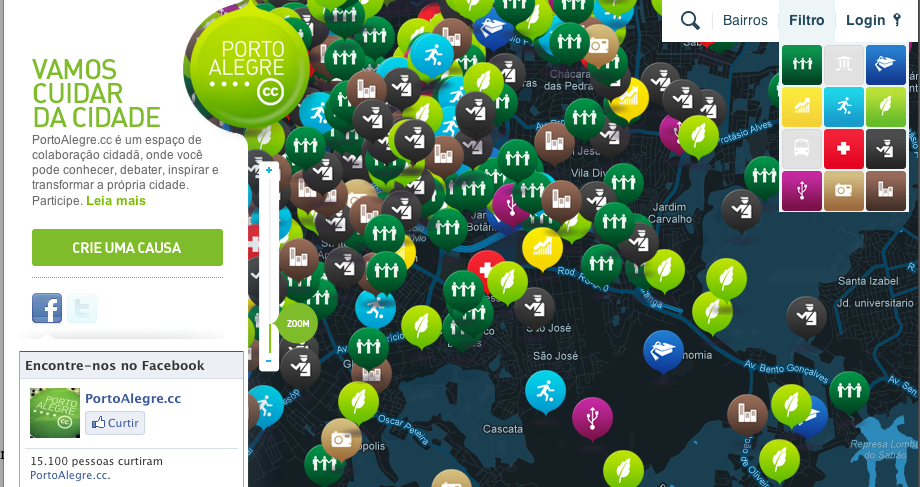
\includegraphics[scale=0.4]{portoalegre-cc}
	\end{center}
	\legend{Fonte: \citeonline{portoalegre}}
\end{figure}

Esse problema fica evidente na \autoref{fig-porto-alegre} quando consideramos, a possibilidade, que um grupo de 5 marcadores reunidos numa região específica, podem sobrepor dezenas ou até milhares de outros marcadores. Ou seja, o mapa não consegue mostrar, com clareza e precisão, as áreas de maior ocorrência de determinado incidente. 

O site fornece um filtro por categorias, que diminui de forma significativa a quantidade de informação exibida.  Mas infelizmente não resolve o problema, pois a sobreposição de informação ainda pode ocorrer com informações de uma mesma categoria.





\subsection{Zoom arbitrário}
Alguns sites criam mecanismos que minimizam o problema da sobreposição de informações. Como exemplo, temos o \citeonline{crimemapatl}  mostrado na \autoref{fig-mapatl} que mostra um mapa com a taxa de crimes em Atlanta. 

O site fornece filtros por categoria, data e zoom. Mas o principal responsável pela eliminação da sobreposição de informação é o filtro por zoom. Esse filtro agrupa todos os marcadores que estão sobrepostos, no zoom atual, em um único marcador que exibe a informação somada dos marcadores que o compõem.
 
\begin{figure}[htb]
	\caption{\label{fig-mapatl} MapATL não possui sobreposição de informação devido ao filtro por zoom}
	\begin{center}
	    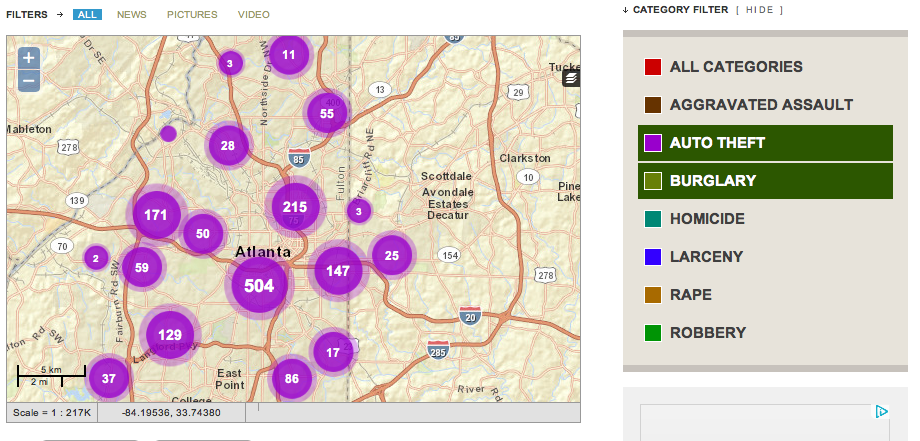
\includegraphics[scale=0.4]{crime-mapatl-com-filtro}
	\end{center}
	\legend{Fonte: \citeonline{crimemapatl}}
\end{figure}

Segundo \cite[42,44]{silva2010solap+} esse tipo de agrupamento, baseado em grelha, pode ser implementado a partir do algorítimo WaveCluster\cite{wavecluster}. 

 

\begin{figure}[htb]
	\caption{\label{fig-zoomab} Entre ZOOM A e ZOOM C existem muitos níveis intermediários e não apenas 1 (ZOOM B).}
	\begin{center}
	    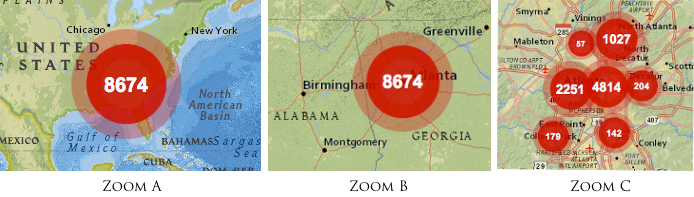
\includegraphics[scale=0.6]{zoomab}
	\end{center}
	\legend{Fonte: \citeonline{crimemapatl}}
\end{figure}

Esse algorítimo resolve o problema de sobreposição de informações. Porém o problema do zoom arbitrário, ilustrado na \autoref{fig-zoomab}, permanece.

O usuário precisa aplicar vários zoons para ir do ZOOM A para o ZOOM C. Mas durante essa interação é gasto tempo e banda, da conexão de internet, do usuário para exibir os zoons intermediários, quando o ideal seria exibir apenas o ZOOM B.

Esse gasto de banda, prejudica a usabilidade de mapas em dispositivos móveis pois, geralmente, eles possuem pouca banda de internet.

Uma abordagem para esse problema é o uso de um zoom inteligente que siga uma hierarquia espacial invés de simplesmente dobrar a visualização atual. 

\subsubsection{Informações arbitrárias}
Um subproblema do zoom arbitrário é a exibição de informações desnecessárias em todos os níveis de zoom. Na \autoref{fig-mapaufes} podemos observar o problema, que neste caso, a arbitrariedade está na exibição de informações, e não no número de zoons. 
 \begin{figure}[htb]
	\caption{\label{fig-mapaufes}Informações necessárias em níveis superiores, de zoom, visualizadas em níveis inferiores}
	\begin{center}
	    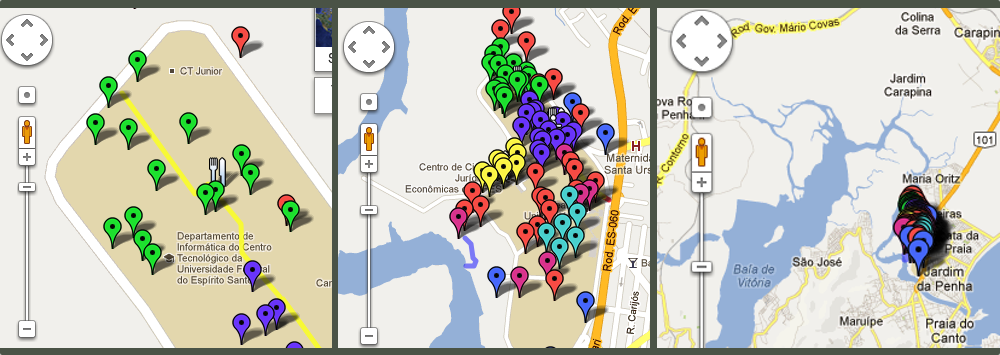
\includegraphics[scale=0.4]{ufes_map}
	\end{center}
	\legend{Fonte: http://maps.google.com}
\end{figure}
Os marcadores desse mapa exibem informações sobre os departamentos internos da UFES, mas essas informações são úteis apenas em certos níveis de zoom. Em níveis mais baixos, onde a área dessa universidade seja desprezível, a informação perde seu valor e fica poluindo o mapa. Neste caso, um único marcador representando o grupo seria mais útil.

\section{Objetivos}
Com base nas informações da definição do problema, o objetivo deste trabalho é desenvolver uma ferramenta que: agrupe marcadores de forma inteligente eliminando a sobreposição; forneça um zoom inteligente que não exiba níveis intermediários desnecessários; esconda marcadores quando sua informação não seja mais necessária ao nível observado.

O objetivo principal desse trabalho é facilitar a visualização de informação em mapas crowdsourcing. Isso devido a importância sócio-econômica das informações que geralmente são exibidas nessa classe de mapas. Mas a ferramenta poderia implementar recursos que também facilite a divulgação dessas informações. Por isso, o objetivo secundário é fornecer um mecanismo para gerar mapas a partir de planilhas de dados, e compartilhá-los sem que o autor precise programar ou ter algum conhecimento de programação. Para este trabalho a divulgação dos mapas é um objetivo secundário, mas poderia ser melhor abordado em trabalhos futuros.
  
\section{Contribuições}
A contribuição deste trabalho é o desenvolvimento de um framework para exibição de mapas em paginas web facilitando a visualização de informações crowdsourcing.

Além disso também foi criado um website do projeto\cite{gitsite} que explica e documenta o framework. O website fornece também um pagina de geração e compartilhamento de mapas por pessoas que não sabem programar.

\section{Estrutura da Monografia}
Este trabalho está organizado da seguinte forma:

Nesta introdução, é apresentado o contexto geral do projeto, a definição do problema, a solução proposta e a estrutura da monografia.

No capítulo 2, Fundamentação Teórica, apresenta-se uma explicação básica sobre os elementos comuns em mapas geográficos, usados na web, e suas relações com crowdsourcing; uma pesquisa sobre as estratégias para lidar com mapas que possuem muitos marcadores; uma pesquisa sobre algorítimos para agrupamento de pontos; uma revisão sobre o uso de planilhas eletrônicas como principal ambiente de programação para usuários finais em órgãos governamentais e seus usos como base de dados para informações geográficas.

No capítulo 3, Desenvolvimento, é explicado como o projeto foi desenvolvido, quais foram as ferramentas utilizadas, e o motivo da escolha de determinadas tecnologias. 

No capítulo 4, Solução Desenvolvida, é apresentado em detalhes a solução que foi desenvolvida e como utilizá-la.

No capitulo 5, Conclusão, é apresentado as dificuldades encontradas no decorrer do projeto, trabalhos futuros e conclusão geral sobre o projeto.






\section{Fundamentos de Mapas Web}
	
	\subsection{Coordenadas Geográficas}
	Coordenadas geográficas são usadas para expressar localizações no mundo. Existem vários sistemas de coordenadas diferentes. O sistema de coordenadas usado pelo Google Maps é o Word Geodetic System 84 (WGS84), que é o mesmo sistema que o Global Position System(GPS) usa.
	
	As coordenadas são expressas usando o conceito de latitude e longitude. Onde latitude mede do sul ao norte e longitude mede do oeste para o leste. No equador a latitude é 0. Isso significa que tudo abaixo do equador (hemisfério sul) possui uma latitude negativa, e tudo acima possui uma latitude positiva. Similarmente também existe uma linha zero para longitude. Ela é conhecida como meridiano, e por razões históricas passa por Greenwich, Inglaterra. Cada posição que é localizada a leste desta linha tem um número positivo e tudo a oeste tem um número negativo\cite[4]{livroGoogleApiV3}. 
	
	A \autoref{fig-coordenadas} permite uma melhor observação desses conceitos:
	\begin{figure}[htb]
	\caption{\label{fig-coordenadas} O centro do mundo na latitude 0 e longitude 0 reside em algum lugar a oeste da costa da África}
	\begin{center}
	    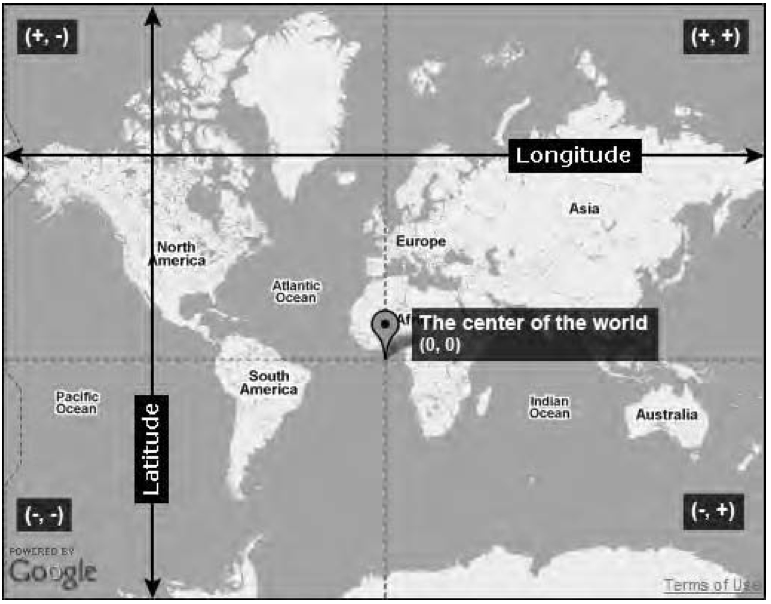
\includegraphics[scale=0.5]{goo-coordenadas}
	\end{center}
	\legend{Fonte: \cite[5]{livroGoogleApiV3}}
	\end{figure}
	
	Dessa forma é possível representar o mapa do mundo em uma imagem retangular que é projetada sobre o plano cartesiano.
	
	Caso seja necessário um maior grau de detalhamento, do mapa, basta que se aumente a resolução da imagem mantendo as proporções e relações entre as coordenadas (x,y), do plano cartesiano, com as coordenadas (longitude, latitude) que são usadas pelo mapa.
		
	\subsection{Zoom}
	As coordenadas de longitude e latitude servem para localizar um ponto numa imagem retangular, através de suas correspondentes x e y do plano cartesiano. Porém mapas também fornecem uma terceira coordenada conhecida como coordenada de Zoom.
	
	 Esta  coordenada controla qual o tamanho da imagem que será usada para projetar o mapa sobre o plano cartesiano. Usualmente, um mapa com coordenada zoom, ou nível de zoom, igual a zero possui uma imagem de tamanho 256x256 pixels. A cada incremento, da coordenada de zoom, dobra-se o tamanho da imagem usada para representar o mapa, e consequentemente o nível de detalhes. De forma que  para zoom=1 a imagem terá 512x512 pixels, para zoom=2 terá 1024x1024 e assim por diante. A \autoref{fig-zoomlevels} exemplifica esse processo:
	\begin{figure}[htb]
	\caption{\label{fig-zoomlevels} A cada incremento de zoom um mapa dobra a sua resolução de imagems}
	\begin{center}
	    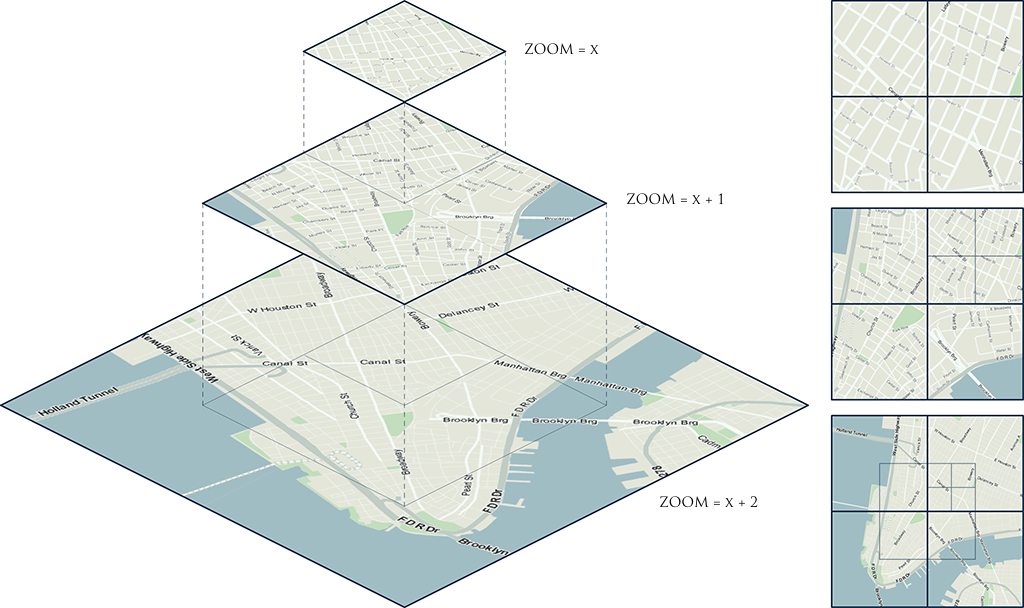
\includegraphics[scale=0.45]{tiles3d}
	\end{center}
	\legend{Fonte: http://workshops.opengeo.org/suiteintro/geowebcache/basics.html}
	\end{figure}

	Portanto para localizar uma posição  em um mapa web, de forma detalhada, precisamos de 3 coordenadas: latitude, longitude e zoom. Além disso, como o tamanho da imagem da projeção varia de acordo com o nível de zoom, o mapa precisa ajustar os valores das coordenadas latitude e longitude para que mantenham suas proporções para os diversos níveis de zoom.

\section{Estratégias para lidar com muitos marcadores}
	Um problema comum, ao se trabalhar com mapas de crowdsourcing, é a enorme quantidade de marcadores necessários para representar os dados do mapa. Isto geralmente afeta a performance do mapa, pois quanto mais marcadores são inseridos mais lenta fica a exibição do mapa. 
	
	É difícil calcular exatamente qual o número máximo de marcadores que um mapa suporta antes de começar a ficar lento, pois a velocidade de exibição do mapa depende tanto do navegador quando do computador em que é exibido. Por exemplo, um mapa pode ser exibido bem rápido em um navegador como o Google Chrome e ao mesmo tempo ser lento quando exibido no Internet Explorer.\cite[177]{livroGoogleApiV3}
	
    Portanto, é necessário um estudo sobre as  estratégias para se lidar com o problema de exibição de muitos marcadores em um mapa. Em \cite[capítulo~9]{livroGoogleApiV3} o autor comenta sobre duas estratégias básicas para esse problema. A primeira e mais óbvia é reduzir o número de marcadores. A segunda estratégia consiste em agrupar os marcadores por algum grau de semelhança.
    
  \subsection{Reduzindo o número de marcadores}
  Existem muitos meios de se reduzir o número de marcadores, entre eles destaca-se as reduções via busca, filtro e otimização visual.
	\subsubsection{Busca}
	Para se reduzir  o número de marcadores exibidos no mapa pode-se fornecer um mecanismo de pesquisa ou busca no mapa. Dessa forma mesmo que o mapa possua milhões de marcadores, somente aqueles que satisfaçam os critérios da busca são exibidos.
	
	 \begin{figure}[htb]
	\caption{\label{fig-estrategiabusca}Busca como estratégia para redução do número de marcadores}
	\begin{center}
	    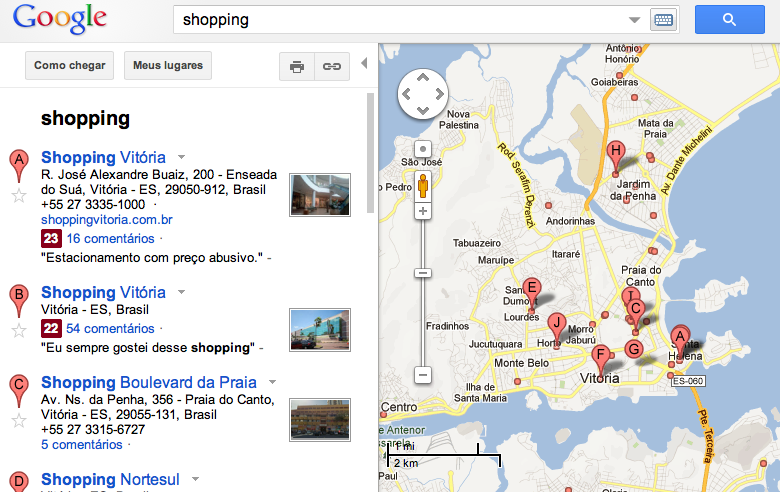
\includegraphics[scale=0.45]{estrategia-busca}
	\end{center}
	\legend{Fonte: http://maps.google.com}
	\end{figure}
	 
	 A \autoref{fig-estrategiabusca}  exemplifica isso ao mostrar o exemplo de busca no google maps. O google maps possui um catálogo enorme de informações, sobre diversas regiões geográficas, mostrar todas essas informações ao mesmo tempo deixaria o mapa muito poluído, e praticamente inutilizável. Como ele implementa o mecanismo de busca isto não acontece.
	
	 Na \autoref{fig-estrategiabusca} observa-se a exibição de uma busca pela palavra chave shopping. Nesta mesma região de interesse existem estabelecimentos de outras categorias como supermercados, lojas, padarias etc. Mas o google maps exibe apenas os marcadores relativos a categoria shopping, que é a palavra chave da busca. Ao fazer isso o mapa fica mais limpo e compreensivo.
	 
	
	\subsubsection{Filtro}
	De forma similar ao mecanismo de busca, um mapa também pode possuir um mecanismo para filtrar grupos de marcadores de acordo com algum critério de seleção do grupo. Dessa forma somente os marcadores que pertençam aos grupos marcados no filtro são exibidos no mapa. 
	
	Diferente do método de busca, este método permite ser mais específico e direto, pois cada campo do filtro é relacionado diretamente com alguma categoria contida nas informações. No método de busca esta relação é menos direta e depende do algorítimo de busca utilizado.  
	
	Como exemplo, ao utilizar-se do método de filtro para marcar 2 categorias, obrigatoriamente, deve ser retornado o resultado para as duas categorias que foram marcadas. Já com o método de busca isto nem sempre é verdade, pois dependendo do algorítimo de busca ele pode entender que a busca por ``categoria 1 categoria 2'' é uma busca por 2 categorias ou uma busca por uma categoria conhecida como ``categoria 1 categoria 1'', que obviamente não seria encontrada. 
	
	A \autoref{fig-estrategiafiltro} mostra um mapa com filtro a esquerda. Observa-se que apenas os marcadores dos grupos  ``Student Housing'' e ``Food/Dining''  são exibidos no mapa.
	 \begin{figure}[htb]
	\caption{\label{fig-estrategiafiltro}Filtro como estratégia para redução do número de marcadores}
	\begin{center}
	    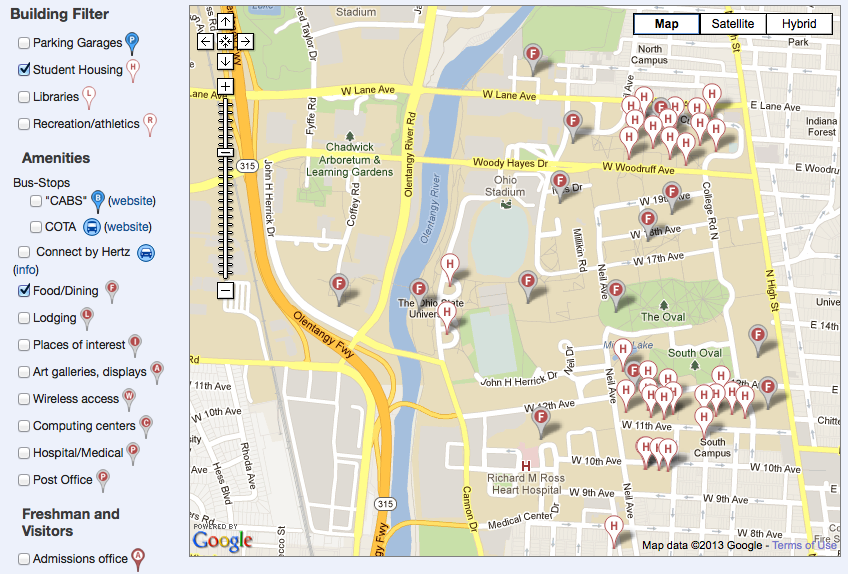
\includegraphics[scale=0.5]{estrategia-filtro}
	\end{center}
	\legend{Fonte: http://www.osu.edu/map/google.php}
	\end{figure}
	 
	\subsubsection{Otimização Visual}
	Nem sempre é preciso usar marcadores para representar dados de um mapa. Em alguns mapas faz mais sentido usar polígonos ou grupo de polígonos para representar um dado ao invés de simplesmente um ponto para o marcador. Por exemplo, ao exibir uma rota  não é necessário um marcador para cada vértice da rota, pois precisa-se apenas do desenho de uma linha, passando por cada vértice, para que a rota seja representada.
	
	A \autoref{fig-otimizacao} mostra um exemplo desse tipo de otimização. No mapa à esquerda, ela exibe uma rota com marcadores em cada vértice do trajeto percorrido. No mapa à direita, ela exibe a mesma rota só que sem colocar marcadores nos vértices do trajeto, deixando apenas um marcador para exibir o ponto de início do trajeto.
	
	 \begin{figure}[htb]
	\caption{\label{fig-otimizacao}Otimização Visual como estratégia para redução do número de marcadores}
	\begin{center}
	    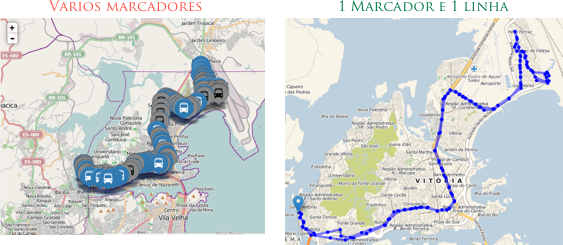
\includegraphics[scale=0.7]{estrategia-otimizacao}
	\end{center}
	\end{figure}
	
	Nesse exemplo, cada vértice da rota representa um ponto de parada para os ônibus que percorrem esse trajeto. Inicialmente, pode se achar necessário a exibição de marcadores nesses vértices como mecanismos de interação com os dados que eles representam. Por exemplo, os usuários do transporte público poderiam querer saber quais são os horários que determinados ônibus passam naquele ponto específico, e com um simples clique no marcador o mapa poderia exibir essa informação. 
	
	Porém, para que este tipo de interação seja possível o mapa teria que exibir os marcadores em cada vértice, que como mostrado na \autoref{fig-otimizacao} não é o melhor caminho. Felizmente, existe algumas alternativas para esse processo que não exigem a presença de um marcador. Por exemplo, ao clicar na linha da rota o mapa pode fazer uma busca, baseada em proximidade, e localizar o ponto que o usuário deseja saber mais informações. Após isso o mapa pode até exibir um marcador temporário como reforço visual do local que está sendo exibida a informação.
	

  \subsection{Agrupamento/Clustering\label{secagrupamento}}
  A segunda estratégia citada por \cite[capítulo~9]{livroGoogleApiV3} para reduzir o número de informações exibidas por um mapa, é conhecida como clustering, ou em português, agrupamento.
  
  A estratégia de agrupamento de marcadores consiste em agrupar marcadores que estejam próximos, por algum critério de proximidade, e exibir apenas 1 marcador para cada grupo e 1 marcador para cada marcador individual, que não pertença a nenhum grupo. Ou seja, em vez de exibir um marcador individual para cada marcador são exibidos marcadores para grupos e marcadores individuais. 
  
  Nessa estratégia os grupos variam de acordo com o zoom. Ou seja, ao fazer zoom em grupo, o grupo se divide em subgrupos menores e, se for o caso, em marcadores individuais.
  
   O processo contrário também ocorre ao diminuirmos o zoom de um grupo. Neste caso o grupo pode se agrupar com grupos vizinhos e formar um novo grupo como mais elementos, de forma, que em alguns mapas, no zoom=0 o mapa exibe apenas 1 marcador representando o grupo com todos os marcadores do mapa.

   Existem diversos métodos para agrupamento de marcadores, mas os mais comuns são implementados usando algum dos seguintes parâmetros para agrupamento: agrupamento por grade, por distancia, ou por região.
     
		\subsubsection{Agrupamento Por Grade}
		Agrupamento baseado em grade é provavelmente a abordagem mais comum para agrupar marcadores. Esta abordagem, divide o mapa em uma grade e agrupa todos os marcadores de cada quadrado em um grupo. 
		
		Apesar de ser uma técnica eficiente, ela possui limitações óbvias, pois pode levar a resultados indesejados. Por exemplo, considere 2 marcadores próximos mas localizados em quadrados diferentes da grade. Neste caso, eles não serão agrupados no mesmo grupo. Para ficar mais claro, veja a \autoref{fig-porgrelha}. 

\begin{figure}[htb]
	\caption{\label{fig-porgrelha}Estes 2 marcadores não serão agrupados pois residem em quadrados diferentes da grade}
	\begin{center}
	    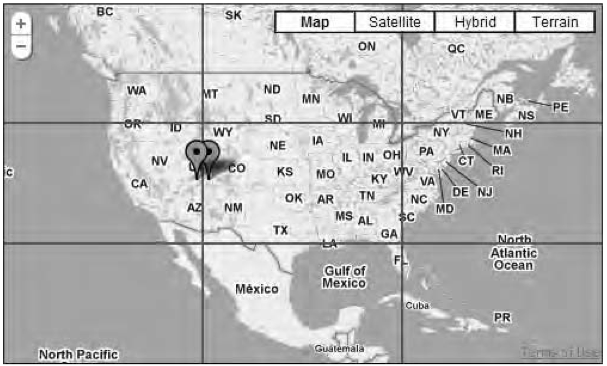
\includegraphics[scale=0.7]{porgrelha}
	\end{center}
		\legend{Fonte: \cite[figura 9.6]{livroGoogleApiV3}}
\end{figure}

		\subsubsection{Agrupamento Por Distância}
			Nesta técnica, não ocorre o problema comentado no agrupamento por grade, pois nela é observado cada marcador e para cada um é procurado marcadores vizinhos, se os marcadores forem próximos o suficiente eles são colocados no mesmo grupo.
		
			Alguns podem achar esta técnica problemática para certos mapas. Pois por agrupar marcadores próximos entre si, os grupos não possuem uma localização fixa como acontece no agrupamento por grade. Assim no agrupamento por distancia os grupos podem aparecer em posições aleatórias que podem não fazer sentido para o usuário que observa o mapa.

		\subsubsection{Agrupamento Por Região}
			No agrupamento por região, define-se diferentes regiões geográficas como países, estados, cidades. E todos os marcadores, de cada região, podem ser agrupados em um grupo para representar a região. Além disso, também é possível definir em que nível de zoom os grupos serão quebrados em subgrupos. 
			
			A vantagem é que fica fácil criar grupos que fazem mais sentido para o usuário. Pois, um agrupamento que siga a ordem Pais > Estado > Cidade é mais natural para o usuário do que um que considere apenas a proximidade.
			
			A desvantagem dessa técnica é o esforço para implementá-la  \cite[182]{livroGoogleApiV3} já que a definição dos grupos não pode ser facilmente automatizada. Essa dificuldade ocorre devido a natureza de como é organizado a hierarquia das regiões, que varia de país para país, sendo necessário em alguns casos o uso de tabelas para conversão\footnote{Até a definição do que é uma autoestrada precisa de uma tabela de conversão entre paises: \url{http://wiki.openstreetmap.org/wiki/Highway:International_equivalence}}.
			
		\subsubsection{Estilos de visualização de agrupamento}
		A representação mais simples de um agrupamento pode ser feita por meio de um marcador. Mas o marcador sozinho não expressa muita informação sobre o grupo, pois não é possível saber a dimensão do grupo olhando para o marcador e muito menos a natureza dos seus elementos. 
		
		Uma alternativa é usar marcadores com tamanhos diferentes de acordo com o tamanho do grupo. Mas, neste caso,tem-se o problema de ter que classificar um tamanho padrão para determinados marcadores. Pode-se, também, usar cores para representar a dimensão do grupo, onde grupos menores tenderiam para o verde e grupos maiores para o vermelho.
		
		Uma solução bastante comum é uma mistura das soluções anteriores. Onde usa-se um marcador com tamanho diferente de acordo com o numero de elementos e cores para maximizar a percepção. Além disso, acrescenta-se uma legenda exibindo o número total de elementos do grupo. Veja a \autoref{fig-visual-agrupamento}
		
		
\begin{figure}[htb]
	\caption{\label{fig-visual-agrupamento}Usando tamanho e cor do marcador para representar a dimensão do grupo}
	\begin{center}
	    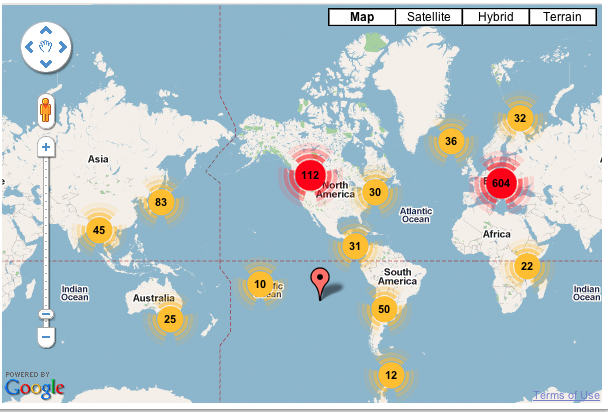
\includegraphics[scale=0.5]{visual-agrupamento}
	\end{center}
		\legend{Fonte: \url{https://developers.google.com/maps/articles/toomanymarkers}}
\end{figure}

	Alguns mapas, possuem dados que permitem uma visualização mais complexa. Para esses tipos de mapa é possível substituir o marcador por uma imagem, gráfico ou forma que represente o grupo.  Por exemplo, uma mapa que mostre as compras de todos os clientes de uma rede de supermercados poderia agrupar os dados inicialmente por loja e na visualização exibir um gráfico de vendas para representar cada grupo. Veja a \autoref{fig-mapa-graficos}.
	
\begin{figure}[htb]
	\caption{\label{fig-mapa-graficos}Usando gráficos para representar agrupamentos}
	\begin{center}
	    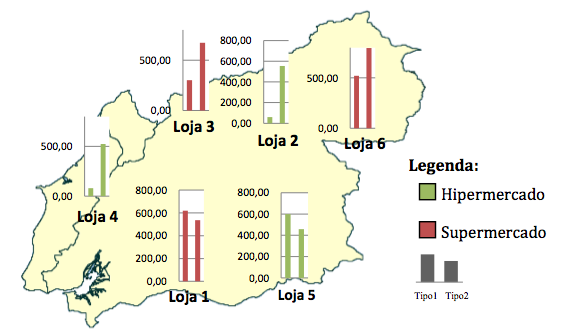
\includegraphics[scale=0.5]{mapa-graficos}
	\end{center}
		\legend{Fonte: \cite[figura 65]{silva2010solap+}  }
\end{figure}

	Além disso, os gerentes dessas lojas,  poderiam efetuar um zoom no gráfico da loja que gerenciam e ver os subgrupos divididos por bairros, com cada grupo exibindo o gráfico de vendas do bairro, permitindo aos gerentes a criação de uma estratégia de marketing localizada.
	
\section{Algorítimos de agrupamento}	
	Basicamente os algorítimos de agrupamentos de pontos podem ser classificados em quatro categorias: (i) método por partição (ii) método hierárquico (iii) método baseado em densidade (iv) método baseado em grade. Isto é ilustrado na \autoref{fig-algoritimos} onde SILVA destaca os potenciais melhores algorítimos para este tipo de problema. Com exceção dos algorítimos k-Means e k-Medoid que foram introduzidos apenas por motivos históricos \cite[35]{silva2010solap+}.
	
	Observa-se que em \cite[capítulo 2]{silva2010solap+} é feito um estudo mais aprofundado sobre os principais algorítimos de agrupamentos de pontos. Por isso, nesta seção será descrito apenas o algorítimo que engloba o contexto deste trabalho. Ou seja, o algorítimo WaveCluster que é baseado no método de grade. 
		
\begin{figure}[htb]
	\caption{\label{fig-algoritimos}Principais algorítimos de agrupamentos de pontos}
	\begin{center}
	    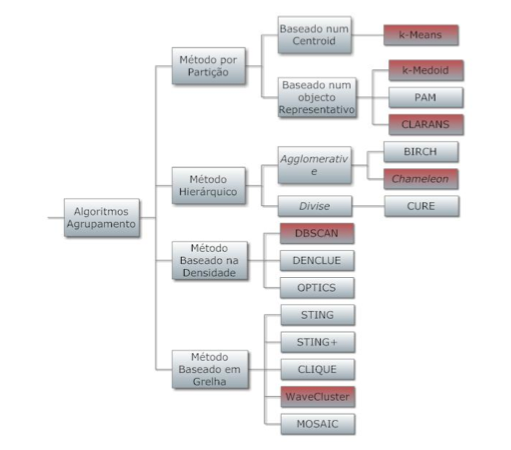
\includegraphics[scale=0.8]{algoritimos}
	\end{center}
		\legend{Fonte: \cite[figura 15]{silva2010solap+}  }
\end{figure}

		\subsection{Métodos baseados em grade}
		Como já foi comentado na \autoref{secagrupamento}, agrupamentos baseados em grade são aqueles que dividem o espaço do mapa em uma grade e agrupa os marcadores de cada quadrado ou célula da grade.  Ou seja, algorítimos baseados em grade são aqueles que usam o agrupamento por grade como parâmetro de agrupamento. 
		Pode se observar na \autoref{fig-algoritimos} que os principais algorítimos são: STING, STING+, CLIQUE, WaveCluster e MOSAIC. E, apesar de não ser o mais indicado para o contexto SOLAP+ que SILVA estudava, o melhor entre os algorítimos baseados em grade é o WaveCluster.
		
		
		\subsubsection{WaveCluster}
			Uma boa abordagem para agrupamentos deve ser eficiente e detectar grupos de formas arbitrárias. Ela também tem que ser insensível a dados discrepantes e a ordem de entrada dos dados.
			
			O algorítimo WaveCluster atende todos esses requisitos. Sua definição completa é encontrada em \cite{wavecluster} mas em resumo o algorítimo faz o seguinte:
\begin{algorithm}
\caption{WaveCluster}
\textbf{Entrada} Vetores de características dos objetos de dados multidimensionais

\textbf{Saida} Objetos agrupados
\begin{enumerate}
\item Quantizar o espaço de características, atribuir objetos as celulas da grade.
\item Aplicar a transformação $wavelet^1$ no espaço de características quantizado.
\item Encontrar os componentes conectados (clusters) nas sub-bandas
\item Transformar o espaço original, em diferentes níveis.
\item Atribuir rótulos as células.
\item Criar a tabela de pesquisa.
\item Mapear objetos aos clusters/grupos.
\end{enumerate}
\end{algorithm}
\footnotetext{Uma transformada de wavelet é uma tecnica de processamento de sinais que decompõe o sinal em diferentes sub-bandas de frequencia.} 

O WaveCluster possui complexidade O(n). Além disso, por causa do uso das técnicas de processamento de sinais a propriedade de multi-resolução, ou agrupamento nos níveis hierárquicos, também é aplicada ao WaveCluster.

O seu uso não é limitado apenas à dados espaciais, o algorítimo WaveCluster pode ser aplicado a qualquer conjunto de atributos com valores numéricos ordenados.
	
%
%
%\section{Planilhas eletrônicas e Mapas}
%\subsection{Domínios de conhecimento}
%Mostra a importância do uso de planilhas \cite{credinePlanilha} 
%\subsection{O desafio chinês}
%mostra o uso de planilhas pelo governo chines e as dificuldades encontradas \cite{chinaPlanilha}
%
%\subsection{Usando planilhas como fonte de dados para Mapas Geográficos}
%Mostra \cite{lieberman2009spatio}

% -------------------------------------
Neste capítulo será detalhado o processo de desenvolvimento do framework Searchlight, e as ferramentas utilizadas para a construção do mesmo.

\section{Considerações Iniciais}
Durante  a fase de pesquisa deste projeto, descobriu-se uma variedade de recursos que poderiam ser usados na elaboração de um framework para visualização de mapas. Muitos destes recursos já estavam no cronograma do projeto, outros foram adicionados  e alguns ficaram fora do cronograma e colocados na lista de trabalhos futuros.

Inicialmente a meta do framework era apenas encontrar uma maneira de visualizar mapas de crowdsourcing de forma mais limpa e sucinta através de técnicas de agrupamento aliadas a hierarquia de zoom. Mas no decorrer das pesquisas percebeu-se que seria interessante adicionar alguns recursos como filtro por categoria e foco em grupo. 

Também foi adicionado ao projeto a possibilidade de gerar e compartilhar um mapa web sem precisar escrever uma linha de código.
O único requisito é fornecer um endereço web onde o gerador de mapas deve buscar os dados geográficos do mapa. Neste caso, o usuário não precisa mais saber programar para poder usufruir dos recursos do framework e a única preocupação dele fica depositada sobre o conteúdo do mapa.

Em relação ao conteúdo usado pelo compartilhador de mapas, o framework atualmente suporta o armazenamento numa planilha eletrônica ou em um arquivo de formato JSON\footnote{Formato muito usado para troca de dados entre websites \url{http://www.json.org}}. Quando o conteúdo é oriundo de planilha eletrônica é necessário que esta esteja armazenada no Google Docs e seja pública. De forma similar, quando o conteúdo é armazenado em um arquivo JSON é necessário que o website que hospeda o arquivo suporte o protocolo JSONP. Caso contrário, o usuário deve instalar o framework Searchlight no website que deseja visualizar o mapa.


Em relação as ferramentas que foram utilizadas no projeto, o objetivo inicial era usar a api do Google Maps para a visualização dos mapas. Porém,  na época em que esta pesquisa era feita, circulava notícias que o Google estaria mudando seus termos de serviço e iria começar a cobrar\footnote{Uma notícia sobre o inicio das cobranças do Google Maps \url{http://goo.gl/f1E3K}} pelo uso da API do Google Maps. Além disso, no mesmo período, a Apple anunciou que iria abandonar o uso do Google Maps em seus smartphones e adotaria uma solução própria. Isto trouxe a necessidade de procurar uma alternativa ao Google Maps, e a alternativa encontrada foi a biblioteca open-source \textbf{Leaflet.js} que será descrita no decorrer deste capítulo.




\section{Ferramentas e bibliotecas us	tilizadas}

Um framework, em desenvolvimento de software, é uma abstração que une códigos comuns entre vários projetos de software provendo uma funcionalidade genérica. Um framework pode atingir uma funcionalidade específica, por configuração, durante a programação de uma aplicação. Ao contrário das bibliotecas, é o framework quem dita o fluxo de controle da aplicação, chamado de Inversão de Controle\footnote{Definição completa em: \url{http://pt.wikipedia.org/wiki/Framework}}.

De modo geral, um framework é conjunto de ferramentas que trabalham em conjunto. O que une as ferramentas são as regras do framework que tem como objetivo prover as funcionalidades que motivaram a criação do framework.

O framework Searchlight tem como objetivo facilitar a criação e a visualização de mapas de crowdsourcing por meio de automatização do processo de criação do mapa. O público alvo abrange tanto  programadores de mapas web quanto  usuários sem nenhum conhecimento de programação. Para atingir este objetivo o framework faz uso do seguinte conjunto de ferramentas: GitHub, Lealflet.js, jQuery, Tabletop.js e RapydScript. 

\subsection{Github}
	
\subsection{GithubPages}

\subsection{Aplicações Comerciais de Agrupamento de Pontos}
		Durante a fase de pesquisa, deste trabalho, foi feito uma busca por aplicações acadêmicas, e comerciais, que já fizessem o uso de algorítimos de agrupamento de pontos. Duas aplicações se destacaram: MarkerClusterer e Leaflet.MarkerCluster.
		\subsubsection{MarkerClusterer}
		
		MarkerClusterer \cite[188]{livroGoogleApiV3} é uma ferramenta fornecida pelo google que estende o uso da API do Google Maps para o uso de algorítimos de agrupamentos.
		
		MarkerClusterer é uma solução baseada em grelha. Ela agrupa marcadores de acordo com sua distância ao centro de um grupo. Quando um marcador é adicionado, ele pesquisa sua posição em todos os grupos. Caso não seja colocado em nenhum grupo, um novo grupo é criado para este marcador. A \autoref{fig-markerclusterer} demonstra a aplicação da ferramenta nos marcadores de um mapa.
	\begin{figure}[htb]
	\caption{\label{fig-markerclusterer}Exemplo de utilização da API MarkerClusterer }
	\begin{center}
	    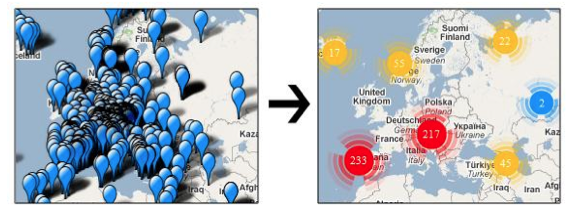
\includegraphics[scale=0.8]{markerclusterer}
	\end{center}
		\legend{Fonte: \cite[figura 20]{silva2010solap+}  }
\end{figure}

		\subsubsection{Leaflet.MarkerCluster}
		Assim como a biblioteca MarkerCLusterer estende a API do Google Maps para uso de agrupamento de marcadores, o plugin Leaflet.MarkerCluster serve como uma extensão para a API, de visualização de mapas, Leaflet.js\footnote{\url{http://leafletjs.com} é uma alternativa  a API do Google Maps, pois fornece um melhor suporte a dispositivos móveis como tablets e smartphones }. 
		
		Este plugin, faz basicamente as mesmas funções da ferramenta MarkerCluster, porém com algumas melhorias. Por exemplo, ao fazer zoom o mapa exibe uma pequena animação do processo de agrupamento; ao se passar o mouse sobre um marcador do grupo o mapa exibe um polígono que mostra os limites alcançados pelo grupo; os grupos que não são visíveis  na visualização atual do mapa são retirados do mapa para aumentar a performance. Além dessas melhorias, uma que merece destaque é a sua incrível capacidade de customização. 

		Ao contrário da biblioteca MarkerClusterer, o plugin Leaflet.MarkerCluster possui um documentação bem completa que pode ser encontrada em \citeonline{gitleafletmaker}. Inicialmente, procurou-se por uma documentação mais abrangente da biblioteca MarkerCluster, mas até o momento da confeção desse trabalho não foi possível encontrar nada além de alguns poucos exemplos de uso. Isto, e outros fatores, contribuíram para a escolha da biblioteca Leaflet.js como API de visualização de mapas do framework Searchlight.
		  
\subsection{Leaflet.js}
\subsection{Leaflet.markercluster}
\subsection{Leaflet.spin}

\subsection{jQuery}
\subsection{jQueryUI}

\subsection{TableTop.js}

\subsection{Rapydscript}


\section{Arquitetura do Sistema}
\subsection{Processamento de dados}
\subsection{Interface com usuário} 
\subsection{Compartilhamento de mapas}
s

Neste capitulo será detalhado o framework Searchlight e os recursos que o mesmo oferece para seus usuários.

\section{Website do projeto}
Pensando em ilustrar os recursos do framework Searchlight, para os usuários do framework, foi criado um website com informações do projeto.

O endereço dele é \url{http://wancharle.github.io/Searchlight/}. Através dele podemos ter acesso ao endereço do código fonte do projeto, que se encontra no GitHub, permitindo assim que outros programadores contribuam para o mesmo.

\begin{figure}[htb]
	\caption{\label{fig-website}Website com documentação e exemplos do framework Searchlight.}
	\begin{center}
	    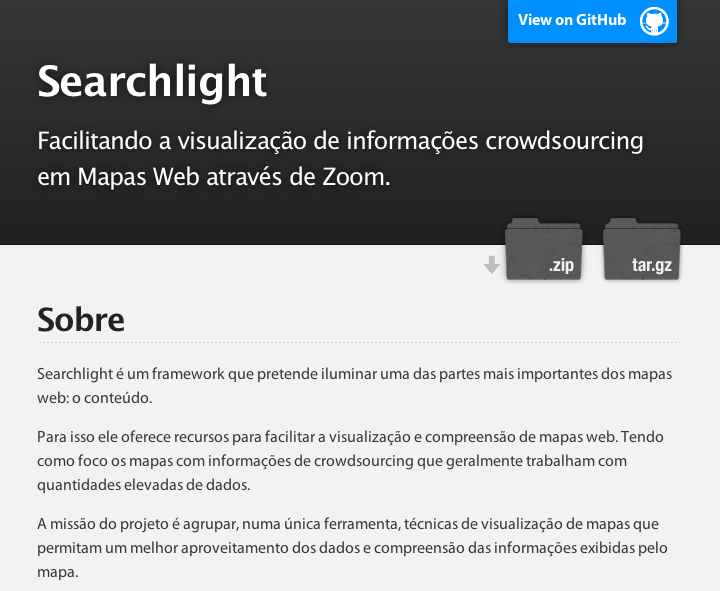
\includegraphics[scale=0.6]{website}
	\end{center}
\end{figure}


Este website contém o link da API Searchlight.js para os programadores que querem utilizar o framework de forma customizada. Nele é possível visualizar exemplos de filtros de categorias, agrupamento de marcadores, foco em grupo, geração automática de mapas e compartilhamento de mapas, que são os principais recursos e meios de utilização do framework. Dentre eles, destacam-se a geração e compartilhamento automático de mapas que possuem páginas específicas para sua utilização. 


Em suma, o website documenta o projeto como um todo. Fala sobre os objetivos e metas do projeto. É possível conferir uma parte do dele na \autoref{fig-website}. 

\section{Recursos desenvolvidos}
A \autoref{sec-estrategias} descreveu duas estratégias que podem ser utilizadas para se lidar com o problema de muitos marcadores num mapa. O framework fornece recursos que se baseiam nessas duas estratégias. 

\subsection{Filtro por categorias}
O filtro por categoria é um dos recursos do framework Searchlight que se baseia na estratégia de redução de marcadores. Através dele é possível selecionar quais categorias de informações devem ser exibidas pelo mapa. 

Para utilizar o filtro por categorias basta que o usuário acesse o menu Searchlight, localizado no campo superior direito do mapa, faça a escolha de quais categorias devem ser exibidas e clique no botão atualizar mapa. 

\begin{figure}[htb]
	\caption{\label{fig-categorias}Filtro por categoria fornecido pelo framework Searchlight}
	\begin{center}
	    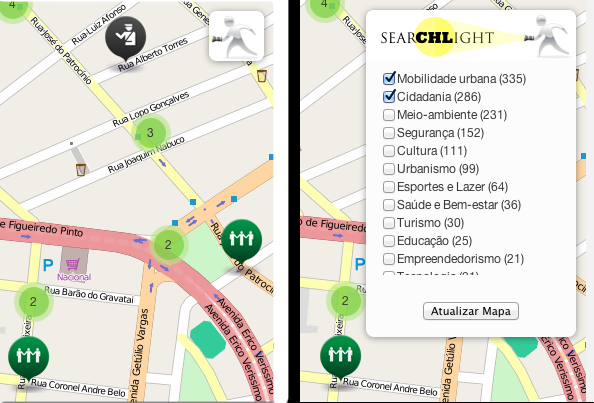
\includegraphics[scale=0.6]{categorias}
	\end{center}
\end{figure}

A \autoref{fig-categorias} exibe o processo de visualização do filtro por categorias.
Como pode ser observado, o filtro  exibe um número ao lado de cada categoria. Este número representa o quantidade de marcadores que pertencem a categoria.

É importante ressaltar, que o filtro de categorias é gerado através da leitura dos dados do mapa. Se os dados utilizados pelo mapa não forem classificados por categoria o filtro não é exibido.

\subsection{Agrupamento de marcadores}	
Outra recurso interessante fornecido pelo framework Searchlight é o agrupamento de marcadores. Por meio, da biblioteca Leaflet.MarkerCluster o framework agrupa os marcadores de acordo com o nível de zoom. Isto resolve somente o problema de sobreposição de informações, que é um dos problemas que motivaram a criação deste projeto. 

Outro problema que também é resolvido pelo agrupamento de marcadores é o problema de zoom arbitrário. Quando o usuário clica em um agrupamento de marcadores o mapa calcula um nível de zoom que possibilita ver todos os subelementos do agrupamento que foi clicado. A \autoref{fig-agrupamentos} exemplifica isso. Com apenas um clique no marcador central o mapa muda do zoom A para o zoom B sem precisar de zoons intermediários como no caso analisado na \autoref{fig-zoomab}.


\begin{figure}[htb]
	\caption{\label{fig-agrupamentos}No framework Searchlight os agrupamentos de marcadores eliminam o zoom arbitrário}
	\begin{center}
	    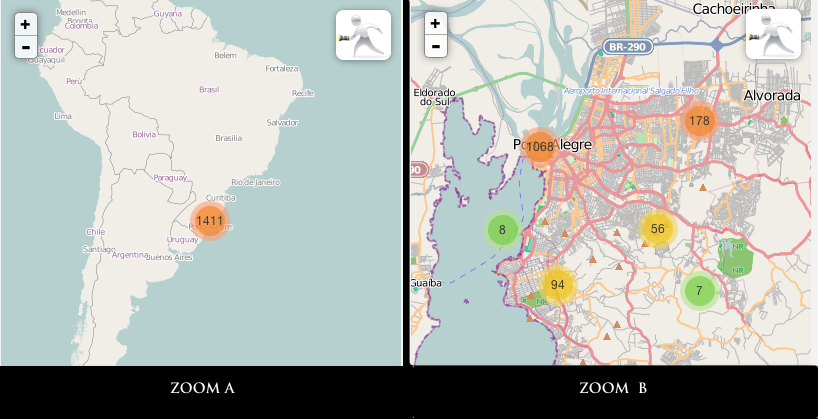
\includegraphics[scale=0.5]{agrupamentos}
	\end{center}
\end{figure}


\subsection{Balões de Resumo e Foco em grupo}
Em mapas com um elevado número de  categorias seria interessante que o framework exibisse algum recurso visual para resumir a informação de cada agrupamento de marcadores. 
No framework Searchlight isto foi implementado através de balões de resumo.

\begin{figure}[htb]
	\caption{\label{fig-baloes}Balões de Resumo do agrupamento clicado}
	\begin{center}
	    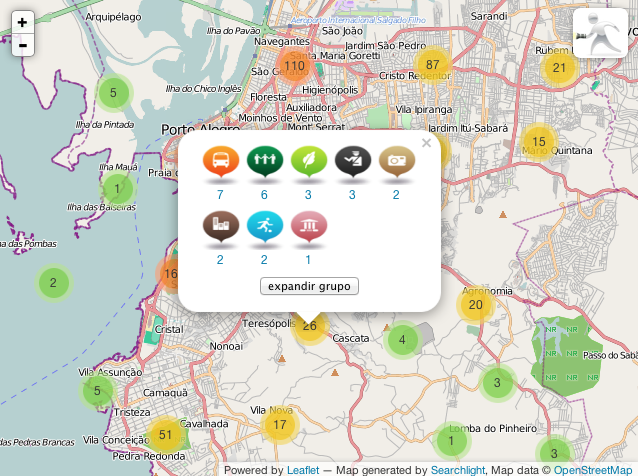
\includegraphics[scale=0.6]{baloes}
	\end{center}
\end{figure}

A \autoref{fig-baloes} exibe um balão de resumo. Como pode se observar, o Balão de resumo mostra um pequeno relatório sobre os elementos pertencentes ao agrupamento. É exibido uma listagem de ícones de categorias que pertencem ao agrupamento que foi clicado, com o total de elementos da categoria a baixo do ícone. 


Balões de Resumo fornecem duas formas de interação. A primeira forma de interação é com o botão ``expandir grupo'' que basicamente faz um zoom no grupo. A segunda forma de interação é com os ícones de categorias. Através dele é possível utilizar o recurso ``Foco em Grupo'' que basicamente faz um zoom no grupo, mas exibindo apenas os elementos pertencentes ao agrupamento e a categoria que foi clicada.

 \begin{figure}[htb]
	\caption{\label{fig-focoemgrupo}Exemplo de Foco em Grupo por categoria segurança}
	\begin{center}
	    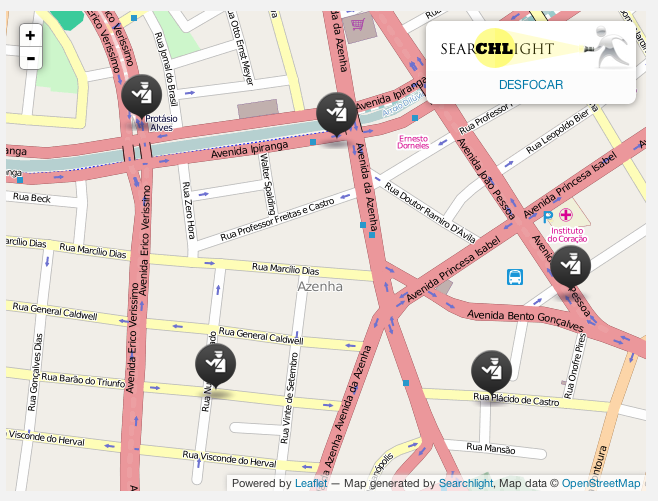
\includegraphics[scale=0.6]{focoemgrupo}
	\end{center}
\end{figure}

O recurso de foco em grupo é útil para situações que se deseja visualizar apenas um tipo de categoria de forma rápida sem que seja preciso marcar e desmarcar categorias no filtro de categorias. Para sair do foco em grupo basta clicar no botão DESFOCAR. Veja \autoref{fig-focoemgrupo}.


\subsection{Geração e Compartilhamento automático de Mapas}
O framework Searchlight permite a geração automática de mapas, através de fontes de dados externas, sem a necessidade de programar o mapa. Para que isso seja possível, convencionou-se que todo objeto de informação terá que conter 3 propriedades essenciais: latitude, longitude e texto.  

As propriedades \textbf{latitude} e \textbf{longitude} são responsáveis por informar a posição em que o marcador deve aparecer no mapa. A propriedade \textbf{texto} é responsável por informar o texto que será exibido no balão do marcador. O conteúdo da propriedade texto pode ser qualquer tipo de texto, inclusive código html.

 A \autoref{fig-fonte} exibe um exemplo de fonte de dados que utiliza a convenção adota pelo framework Searchlight. Neste caso, foi utilizado uma planilha pública do Google Drive e na coluna texto foi colocado  códigos html e texto simples. 		
  
 \begin{figure}[htb]
	\caption{\label{fig-fonte}Exemplo de fonte de dados utilizada para gerar mapas automaticamente}
	\begin{center}
	    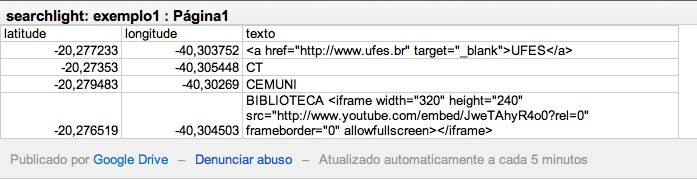
\includegraphics[scale=0.6]{fonte}
	\end{center}
\end{figure}

De modo geral, é necessário criar uma planilha de dados para  gerar um mapa automaticamente. Além disso, é preciso acessar o gerador de mapas no website do projeto e colar o endereço  da planilha no campo ``endereço da planilha''. Por ultimo, deve-se clicar no botão ``compartilhar'' para visualizar o mapa gerado.

É importante perceber, que a fonte de dados não precisa ser necessariamente uma planilha do Google Drive. O framework Searchlight também suporta o formato de dados JSON. E por meio do protocolo JSONP pode usar estes arquivos como fonte dados na geração automática de mapas.  



% ---
% Conclusão
% ---
%\chapter*[Conclusão]{Conclusão}
%\addcontentsline{toc}{chapter}{Conclusão}

Este capítulo apresenta as conclusões do trabalho realizado, mostrando suas contribuições. Por fim, são apresentadas suas limitações e perspectivas de trabalhos futuros.

\section{Conclusões}
Com a popularização dos computadores e da internet, está acontecendo um aumento da interação social entre as pessoas no meio virtual. Essa interação permite o cultivo de novos comportamentos e interações sociais como o crowdsourcing. Além disso, tem crescido a necessidade de mecanismos virtuais que permitam as pessoas exercer sua cidadania de forma conectada e contribuir para a cidade com  criticas e sugestões. Entretanto, tais mecanismos precisam lidar com uma enorme quantidade de informação e isso dificulta a visualização dos dados coletados.

Neste contexto, este trabalho apresentou a criação do framework Searchlight com o intuito de facilitar a visualização de informações crowdsourcing em Mapas Web. Pesquisou-se por estratégias para resolver os problemas de sobreposição de informações, zoom arbitrário e informações arbitrárias. E para solucionar esses problemas, foi necessário utilizar as estratégias de redução de número de marcadores e agrupamento de marcadores.

Para a aplicar essas estratégias, o framework Searchlight implementou alguns recursos como o filtro por categorias, o agrupamento de marcadores, Baloes de Resumo e foco em grupo. Esses recursos, ajudaram a melhorar a visualização do mapa e a deixá-lo mais limpo e compreensível.

Durante a fase de pesquisa, percebeu-se, que além de melhorar a visualização do mapa, era necessário  melhorar também o acesso ao mapa. Para isso, foi feito a implementação do recurso de gerar e compartilhar mapas automaticamente. Com esse recurso, usuários que não possuem conhecimento de programação também podem criar  e compartilhar os seus próprios mapas.



\section{Limitações e Perspectivas Futuras}


No cenário alcançado, algumas limitações são observadas, o que dá margem para a realização de trabalhos futuros. Dentre elas destaca-se o fato da geração automática de mapas aceitar apenas planilhas do Google Docs e não ser possível utilizar planilhas de aplicativos como Excel, Calc e Numbers. Atualmente, o usuário pode adicionar seus dados nesses outros formatos de planilhas, mas para usa-las no mapa  é necessário que elas sejam convertidas para  o formato de planilha do Google Docs.

Além disso, na \autoref{sec-estrategias} foi demostrado que uma das estratégias para se reduzir o número de marcadores é a Otimização visual. Um exemplo de otimização visual genérica que poderia ser implementada no framework é a conexão de marcadores de uma mesmas categoria. Por exemplo, se consideramos um mapa que exibe todos os pontos de ônibus de uma cidade e conectarmos os pontos pertencem a uma mesma linha de ônibus, podemos substituir todos os marcadores do trajeto por um desenho de uma linha passando pela localização dos pontos de ônibus. 

Ainda assim,há espaço para acréscimos de novas funcionalidades  como: filtros por data em mapas temporais, campos de busca em mapas com muita informação textual, e muitas outras.  

Portanto, vislumbra-se a possibilidade de trabalhos futuros objetivando o oferecimento de mais serviços por parte do framework Searchlight e uma melhoria continua dos recursos de visualização de mapas de crowdsourcing.


% ---
% Finaliza a parte no bookmark do PDF, para que se inicie o bookmark na raiz
% ---
\bookmarksetup{startatroot}% 
% ---






% ----------------------------------------------------------
% ELEMENTOS PÓS-TEXTUAIS
% ----------------------------------------------------------
\postextual


% ----------------------------------------------------------
% Referências bibliográficas
% ----------------------------------------------------------
\bibliography{monografia}

% ----------------------------------------------------------
% Glossário
% ----------------------------------------------------------
%
% Consulte o manual da classe abntex2 para orientações sobre o glossário.
%
%\glossary

% ----------------------------------------------------------
% Apêndices
% ----------------------------------------------------------

%% ---
%% Inicia os apêndices
%% ---
%\begin{apendicesenv}
%
%% Imprime uma página indicando o início dos apêndices
%\partapendices
%
%
%\end{apendicesenv}
%% ---
%
%
%% ----------------------------------------------------------
%% Anexos
%% ----------------------------------------------------------
%
%% ---
%% Inicia os anexos
%% ---
%\begin{anexosenv}
%
%% Imprime uma página indicando o início dos anexos
%\partanexos
%
%
%\end{anexosenv}

%---------------------------------------------------------------------
% INDICE REMISSIVO
%---------------------------------------------------------------------

% \cleardoublepage
% \phantomsection 
\printindex

\end{document}
